\chapter{Project setup}\label{Chap:Setup}
In this section will be described the necessary steps to have the application up and running.
\section{Necessary libraries}
The setup of the necessary libraries and framework has been done simmetrically to the one performed in DP2 virtual machine available on the course website. Only difference is the addition of Z3 library for the machine, the setup of it is shown in section \ref{SubSec:Z3Setup}. In figure \ref{Fig:OptFolder} is shown the actual setup used for the machine.
\begin{figure}[!htb]
   \centering
   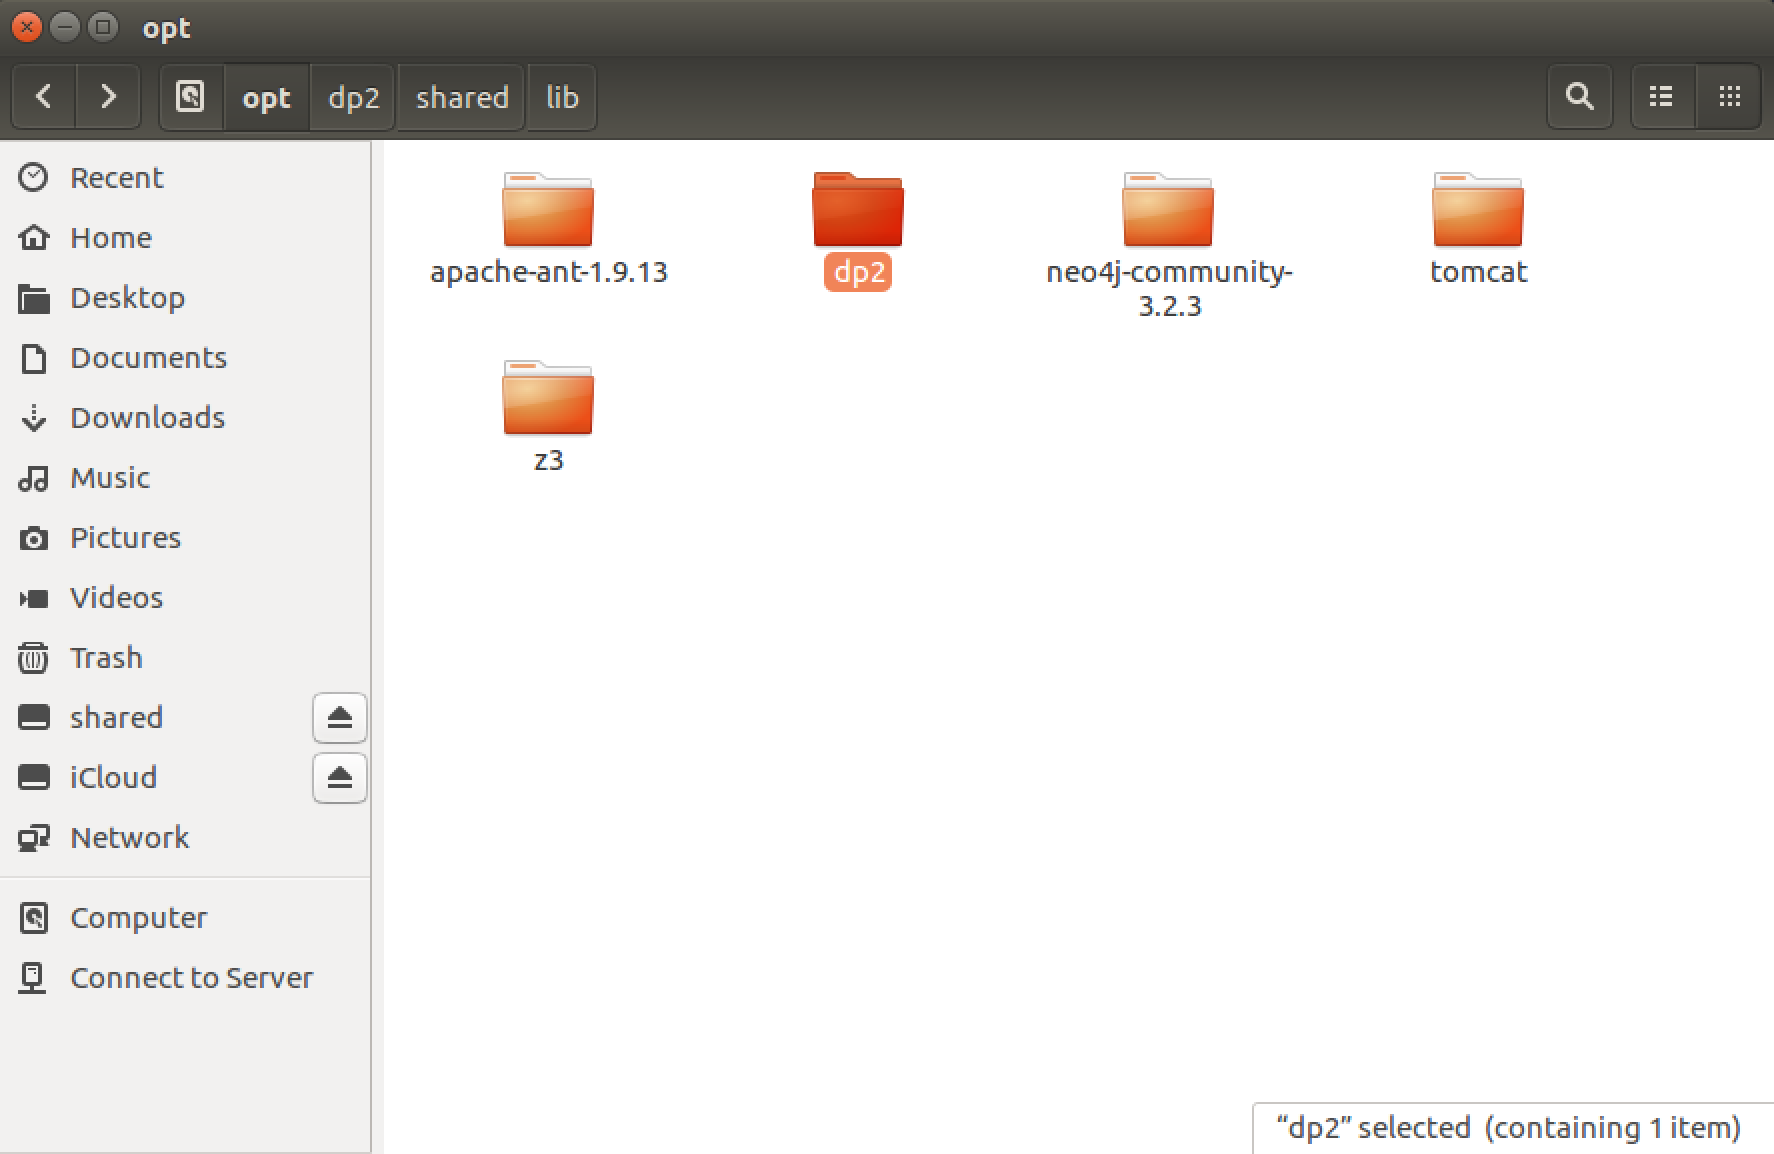
\includegraphics[width=\textwidth]{opt_folder.png}
   \caption{Folder \textit{/opt} of the machine used as development environment.}\label{Fig:OptFolder}
\end{figure}
Additional library like neo4j drivers and junit are provided in the \textit{lib} and \textit{lib-src} folder of the application project. They are already included in classpath during compilation launched through ant scripts. If errors are signaled by Eclipse when opening the project, probably they should be added to build path. After the addition it is suggestable to refresh and clean the project.


% --------------------------------------------------------------------------

\section{Setup of Z3 in machine running Ubuntu}\label{SubSec:Z3Setup}
The development enviroment that has been used is \textbf{Ubuntu}. In order to use Z3 library in such operating system, there are a couple of steps one has to follow.

\begin{enumerate}
	\item \underline{download} the prebuilt version of the library from the offical GitHub repository \url{https://github.com/Z3Prover/z3/releases};
	\item once extracted the files, we have to place them in a specific location in which we will command other applications to look for the needed classes;
	\begin{figure}[!htb]
		\centering
		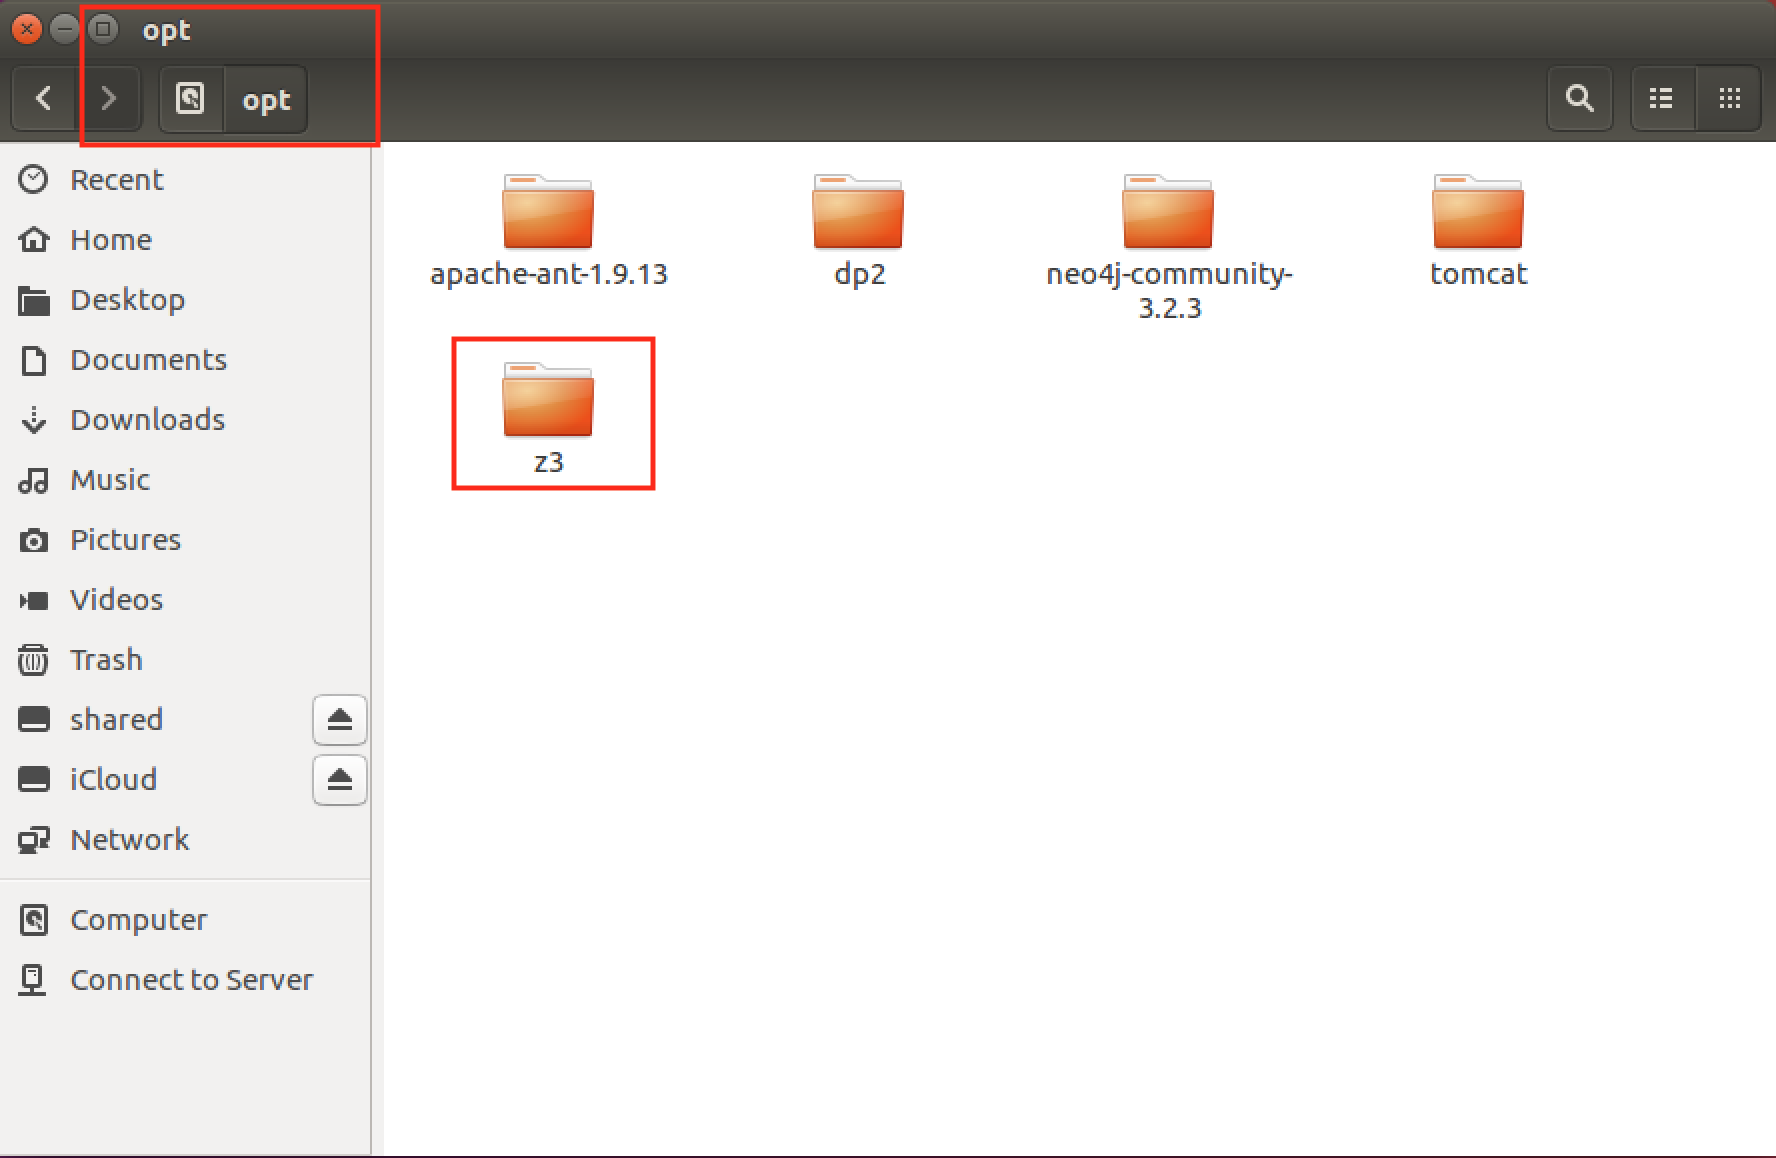
\includegraphics[width=\textwidth]{z3_location.png}
		\caption{Example of where to place Z3 extracted libraries.}\label{Fig:Z3Location}
	\end{figure}
	\item after everything has been placed in the chosen location, we have to \textbf{define} an environment variable which will allow the Java application to know where the Z3 library is located. For Ubuntu such variable is \underline{LD\_LIBRARY\_PATH}. This variable must point to the location of the \underline{bin} folder of the extracted Z3 library;
	\begin{figure}[!htb]
		\centering
		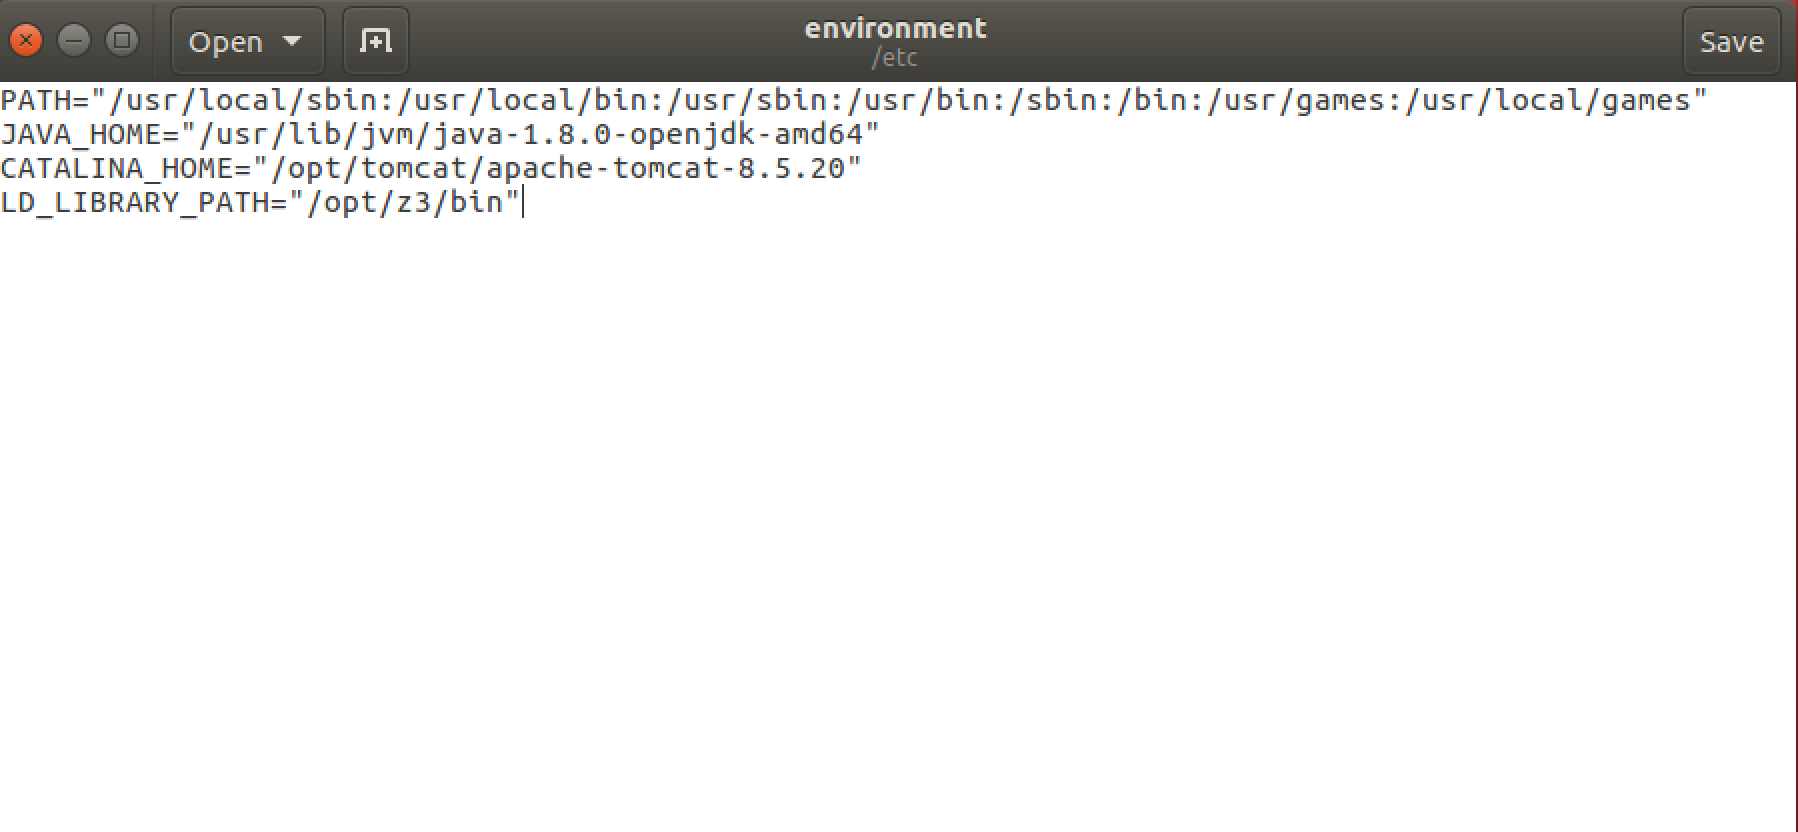
\includegraphics[width=\textwidth]{z3_environment.png}
		\caption{Example of how to define LD\_LIBRARY\_PATH environment variable.}\label{Fig:Z3Environment}
	\end{figure}
	In figure \ref{Fig:Z3Environment} is shown an example of definition of the LD\_LIBRARY\_PATH environment variable. \\
	In this case has been define globally for the whole machine, that means it has been inserted in the file \textit{/etc/environment}, but the same result could have been achieve defining it locally for the used in \textit{/Home/.bashrc} file;
	\item last step, is to add the Z3 .jar file to the build path of our project.
	\begin{figure}[!htb]
		\centering
		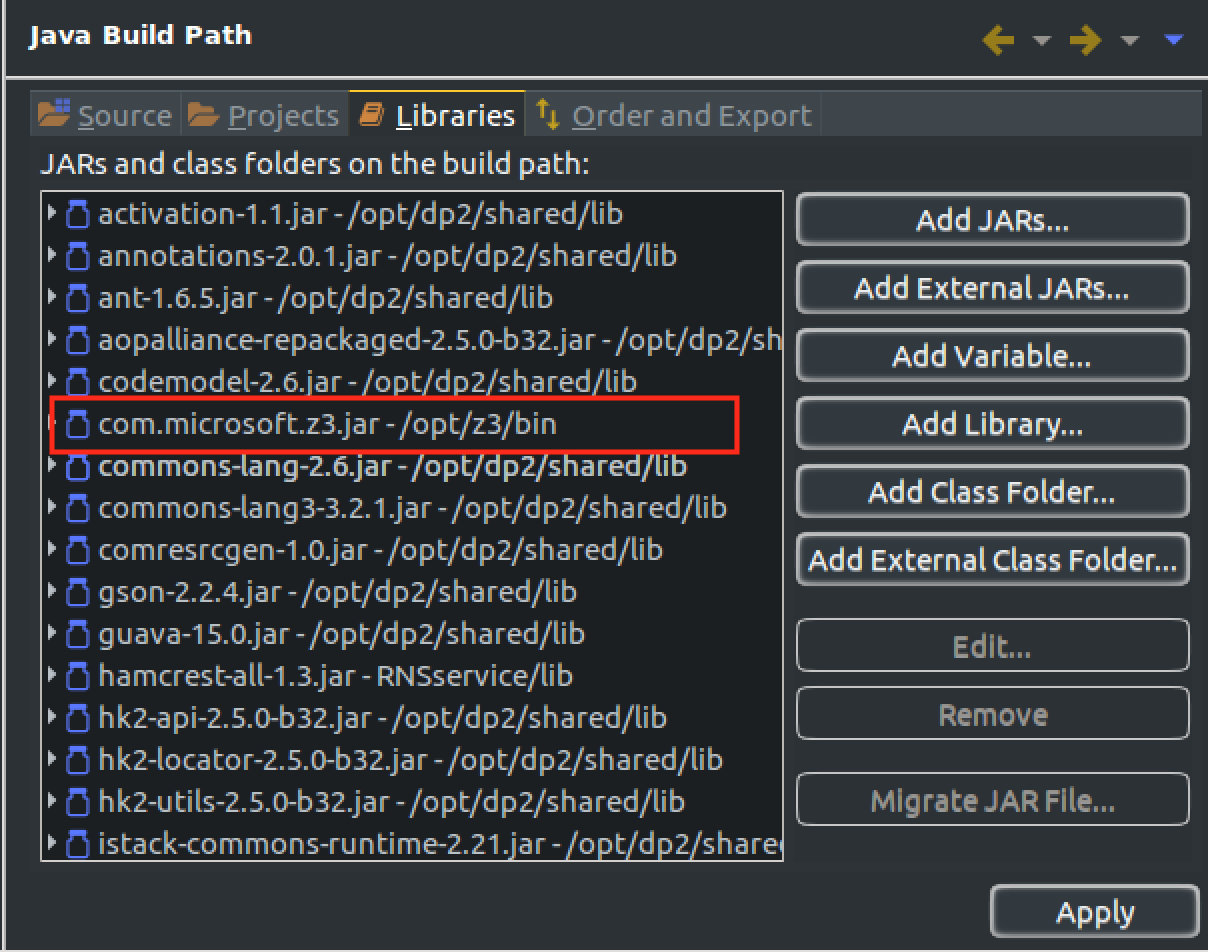
\includegraphics[width=\textwidth]{z3_buildpath.png}
		\caption{Example of how the project build path should look like.}\label{Fig:Z3BuildPath}
	\end{figure}
\end{enumerate}
This is an automatic configuration and Tomcat will load the dynamic libraries in the bin folder by itself. If this is not sufficient, we need to manually put in the WebContent/WEB-INF/lib/jni the Z3 library and point LD\_LIBRARY\_PATH to that folder. Double check that the .jar file is present in the copied folder.\\
Please make sure, in order to use the library in Tomcat, to have correctly set CATALINA\_HOME variable, pointing to Tomcat folder and JAVA\_HOME variable (provided you have installed Java on the machine).

\section{Server application and tests}
In order to launch and compile the server application (in the directory \textit{RNSService}) and its tests,  it is available a set of ant scripts. In particular:
\begin{itemize}
  \item ant script \textbf{neo4j-build.xml} provides a set of target to launch/stop/restart\&clean neo4j database;
  \item ant script \textbf{build.xml} provides all the target to start/stop tomcat, to deploy the application and to run tests, it relies upon another script to define the operation of such targets, that is \textbf{build-rns.xml}.
\end{itemize}
The targets can be either launched via Eclipse IDE or command line. \\
To setup the server up and running it is necessary to follow these step:
\begin{enumerate}
  \item start Neo4j by using \textbf{start-neo4j} target of \textbf{neo4j-build.xml} script. From command line \textit{ant 'start-neo4j' -f /path/to/neo4j-build.xml};
  \item start Tomcat by calling \textbf{start-tomcat} target of \textbf{build.xml} script. From command line \textit{ant 'start-tomcat' -f /path/to/build.xml};
  \item deploy web service by calling \textbf{redeploy} target of \textbf{build.xml} script. From command line \textit{ant 'redeploy' -f /path/to/build.xml}.
\end{enumerate}
This last command embed in itself the generation of the bindings from XML Schema with JAXB and the compilation of all the necessary classes.\\
In order to launch the tests written for the service it is necessary to use \textbf{rns-tests} target of \textbf{build.xml} script. This target will launch the coompilation of all the classes necessary to the tests and launch them with JUnit.

\section{Client application}
To setup the client (in the directory \textit{Client}) it is necessary to install Node.js, then it is possible to launch the application. To get Node.js, go to nodejs.org.
These are the steps:
\begin{enumerate}
	\item go to dir \textit{Client}
	\item install the angular CLI running the following command:\\ \textit{npm install -g @angular/cli} 
	\item get all node dependencies running the following command:\\ \textit{npm install} 
	\item launch the app running the following command:\\ \textit{ng serve}
\end{enumerate}